
\section{Generative Models}
\label{ex:4}


\subsection{Energy-Based Models}
\label{ex:4.1}

\subsubsection*{Restricted Boltzmann Machines}

\begin{task}{4.1.1}
  % In the notebook, the training algorithm refers to the pseudo-likelihood. Why is that? What are
  % the consequences regarding the training procedure?
\end{task}

Pseudo-likelihood is similar to likelihood in the sense that it is a measure of how well the model
fits the data. However, it is not a true likelihood function. Instead, it is a product of
conditional probabilities of each pixel given all other pixels. This makes it easier to compute and
is a good approximation of the true likelihood.


\begin{task}{4.1.2}
  % What is the role of the number of components, learning rate and number of iterations on the
  % performance? You can also evaluate it visually by reconstructing unseen test images.
\end{task}

\begin{figure}[ht]
  \centering
  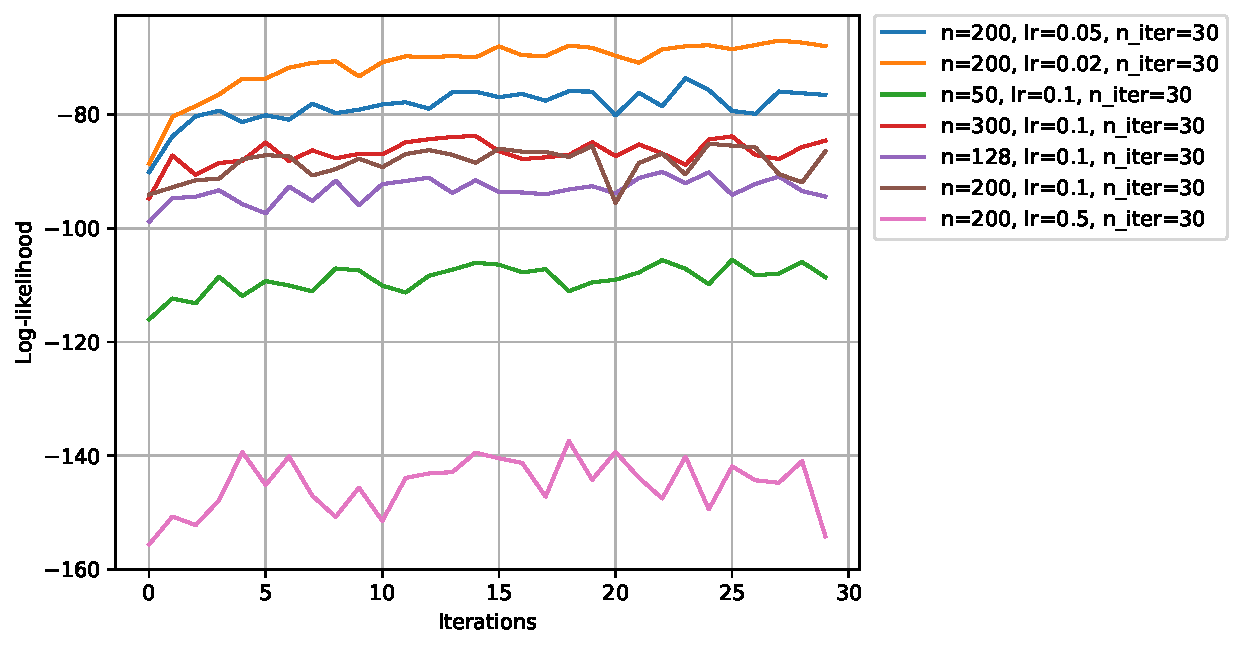
\includegraphics[width=0.9\textwidth]{ex4_1_rbm_likelihoods.pdf}
  \caption{Pseudo-likelihoods of RBM training with different parameters.}
  \label{fig:ex4_1_rbm_likelihoods}
\end{figure}

With a low learning rate, the model converges slowly which would need a higher number of iterations
to reach the same performance. On the other hand, a high learning rate can cause oscillations in the
training process. This can be seen in the variance of the pseudo-likelihood values.\\
The number of components had the biggest impact on the performance. With too few components, the
reconstructed images were blurry and did not resemble the original data. The number of iterations
needed to be big enough for the model to converge. Chosing a higher number of iterations did not
improve the performance significantly. I assumed the model to be converged based on the
pseudo-likelihood values in Figure~\ref{fig:ex4_1_rbm_likelihoods}.\\
The performance of the model was evaluated visually by reconstructing unseen test images. The best
results were achieved with $200$ components, a learning rate of $0.1$, and $30$ iterations.
Counterintuitively, the model produced more convincing results than other models that achieved a
higher pseudo-likelihood. This could be due to the fact that the pseudo-likelihood is not a perfect
measure of the model's performance.


\begin{task}{4.1.3}
  % Change the number of Gibbs sampling steps. Can you explain the result?
\end{task}

\begin{figure}[ht]
  \centering
  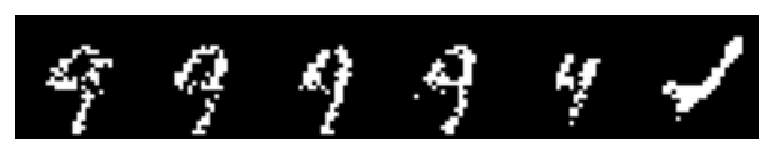
\includegraphics[width=0.9\textwidth]{ex4_1_rbm_gibbs_steps.pdf}
  \caption{Reconstructed images of a $9$ with Gibbs sampling steps. Number of Gibbs sampling steps:
    $1$, $2$, $5$, $10$, $100$, $1000$.}
  \label{fig:ex4_1_rbm_gibbs_steps}
\end{figure}

The effect of the number of Gibbs sampling steps can be seen in
Figure~\ref{fig:ex4_1_rbm_gibbs_steps}. With only one Gibbs sampling step, the model can already
reconstruct the image quite well. With more steps, the image only improves slightly. After more than
$10$ steps, the image degrades and converges to something that could resemble a different digit or
the mean of all digits. This could be related to the problem of iterated functions, where the model
converges to a fixed point.

\begin{task}{4.1.4}
  % Use the RBM to reconstruct missing parts of images. Discuss the results.
\end{task}

\begin{figure}[ht!]
  \centering
  \begin{minipage}{0.48\textwidth}
    \centering
    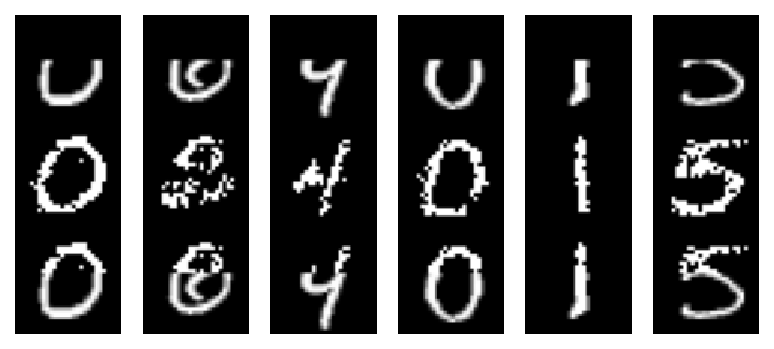
\includegraphics[width=0.9\linewidth]{ex4_1_rbm_reconstruction.pdf}
    \captionof{figure}{Top: Original images with missing parts. Middle: Reconstructed images. Bottom: Merge of original and reconstructed images.}
    \label{fig:ex4_1_rbm_reconstruction}
  \end{minipage}
  \begin{minipage}{0.48\textwidth}
    \centering
    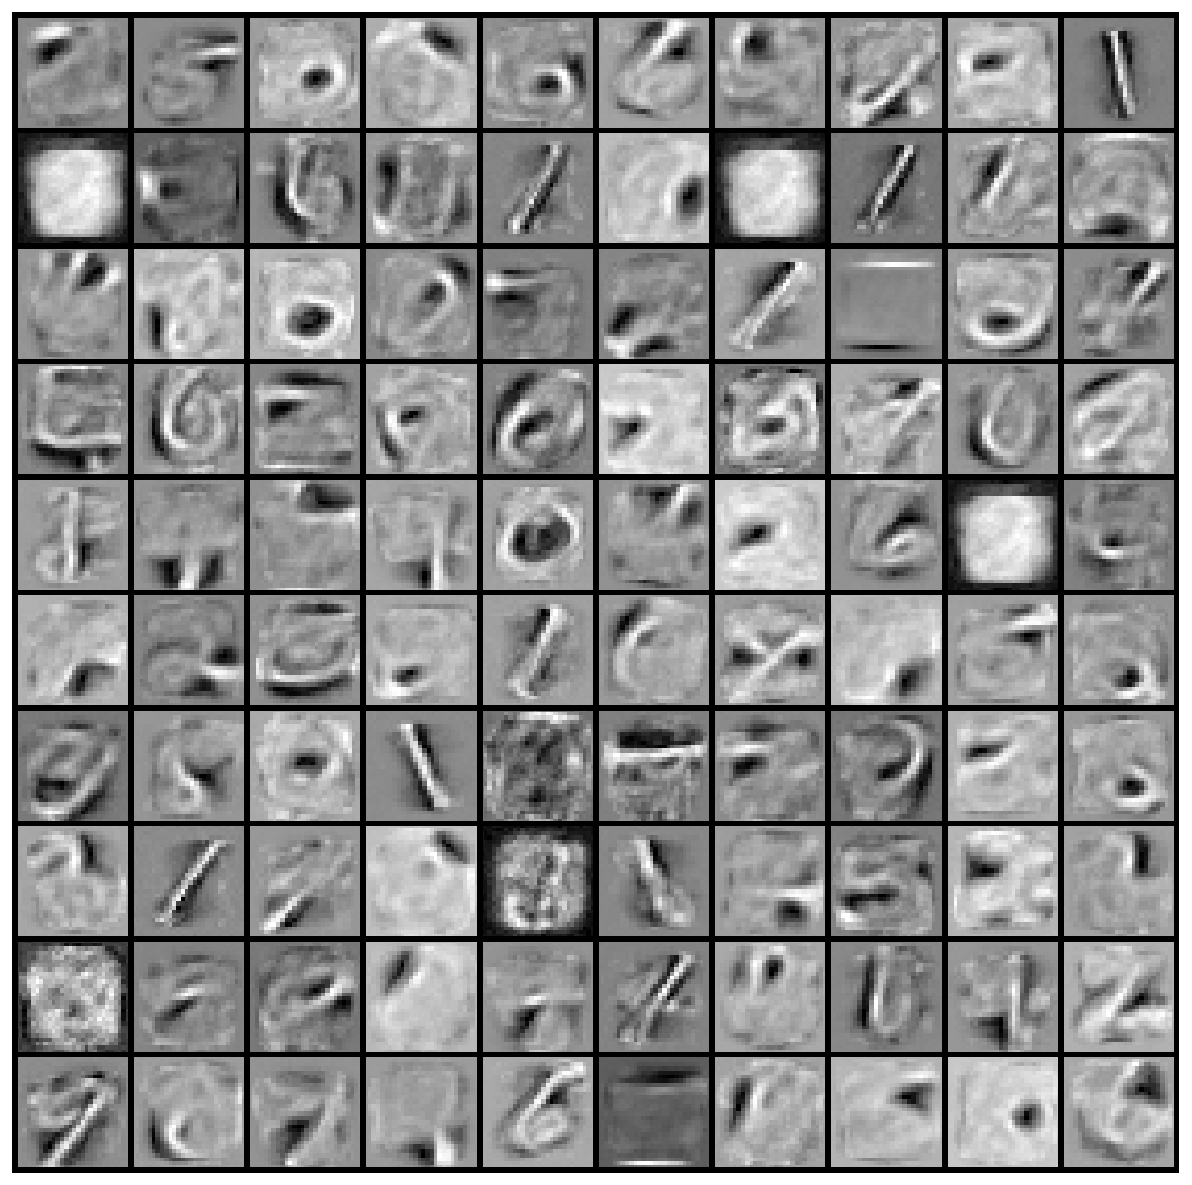
\includegraphics[width=0.9\linewidth]{ex4_1_rbm_components.pdf}
    \captionof{figure}{Components of the RBM.}
    \label{fig:ex4_1_rbm_components}
  \end{minipage}
\end{figure}

In this example, 12 rows at the top of the image were removed. The RBM is able to reconstruct some
digits better than others, as shown in Figure~\ref{fig:ex4_1_rbm_reconstruction}. Two of the
$0$-digits have decent reconstructions. The digit $1$ works particularly well, likely because of its
simple shape. The digit $9$ is falsely reconstructed as a $4$. However, the model manages to
reconstruct the digit $5$ correctly, even though it could also be seen as a $3$ with the top part
missing. In this case, the model has the most trouble with the second $0$-digit, because of the
additional stroke in the middle.


\begin{task}{4.1.5}
  % What is the effect of removing more rows in the image on the ability of the network to
  % reconstruct? What if you remove rows on different locations (top, middle...)?
\end{task}

When removing more rows, the quality of the reconstruction decreases quickly. With $16$ rows
removed, the model only manages to reconstruct about half of the digits correctly. Removing rows on
the bottom, left or right side of the image has a similar effect. With removed rows in the middle,
the model has more trouble, likely because the middle of the image contains more context than the
edges.

\vspace*{0.3cm}
\subsubsection*{Deep Boltzmann Machines}

\begin{task}{4.1.6}
  % Load the pre-trained DBM that is trained on the MNIST database. Show the filters
  % (interconnection weights) extracted from the previously trained RBM (cf. supra) and the DBM,
  % what is the difference? Can you explain the difference between filters of the first and second
  % layer of the DBM?
\end{task}

\begin{figure}[ht]
  \centering
  \begin{subfigure}{0.49\textwidth}
    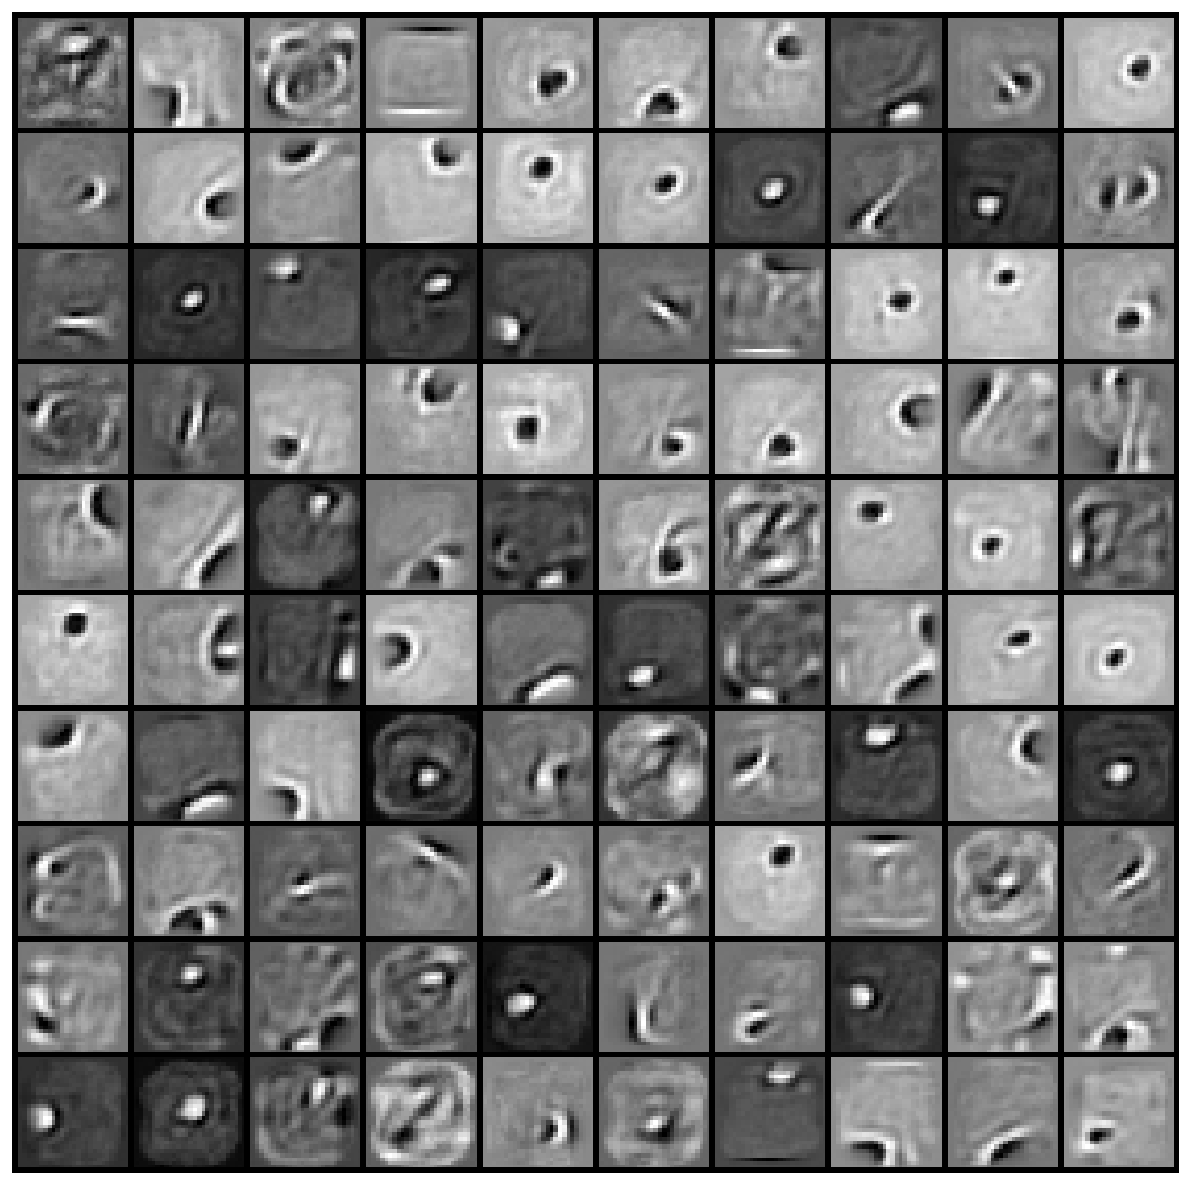
\includegraphics[width=\textwidth]{ex4_1_dbm_components_1.pdf}
    \caption{First layer}
    \label{fig:ex4_1_dbm_components_1}
  \end{subfigure}
  \begin{subfigure}{0.49\textwidth}
    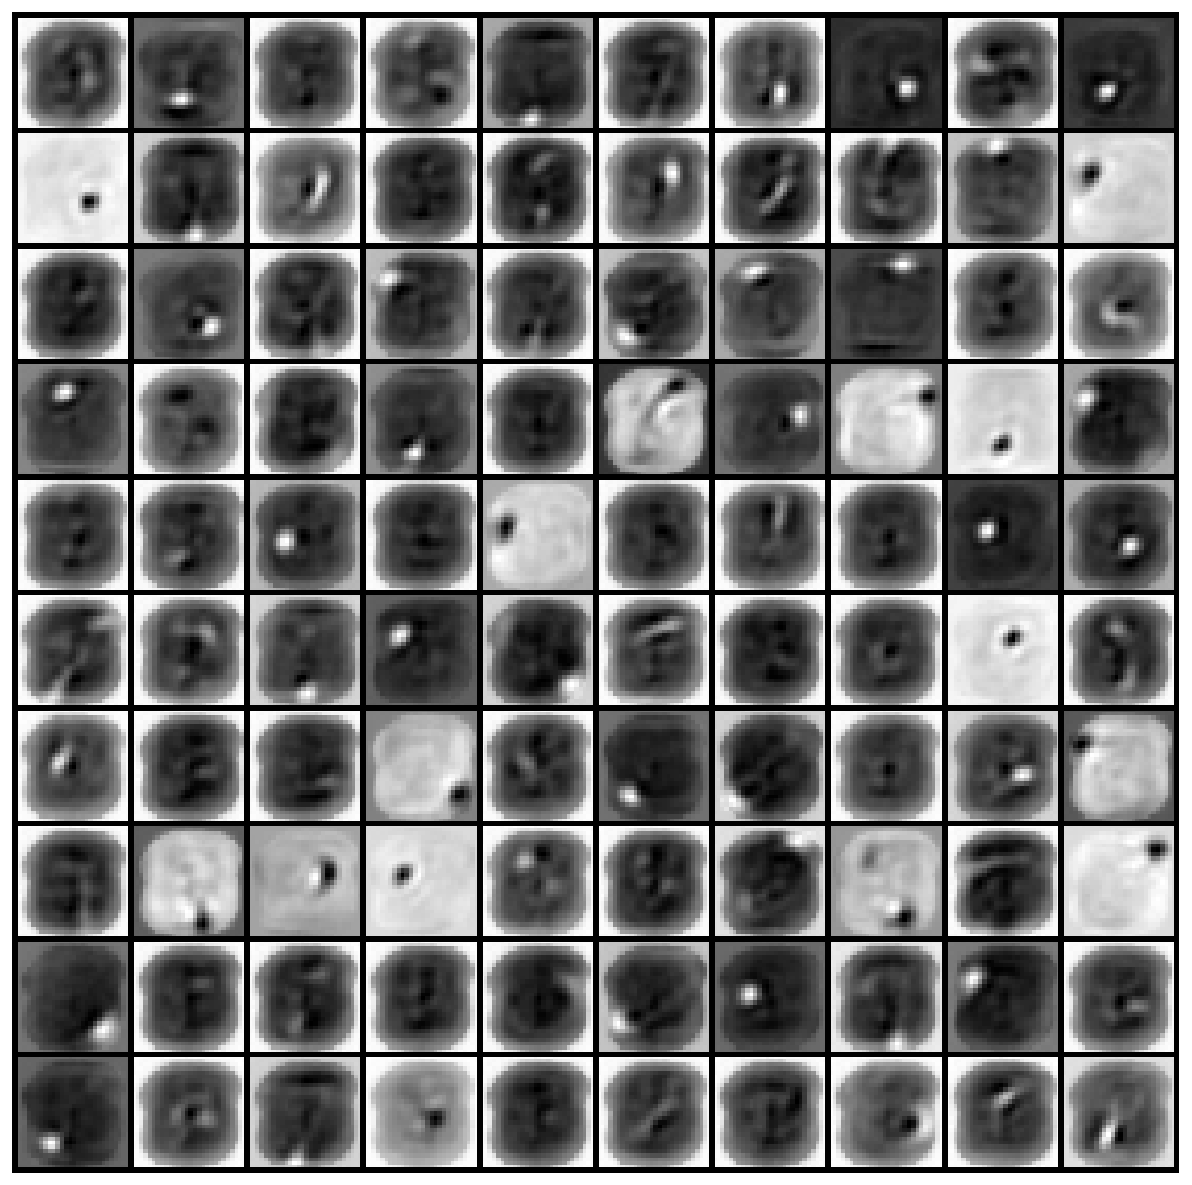
\includegraphics[width=\textwidth]{ex4_1_dbm_components_2.pdf}
    \caption{Second layer}
    \label{fig:ex4_1_dbm_components_2}
  \end{subfigure}
  \caption{Components of the DBM.}
  \label{fig:ex4_1_dbm_components}
\end{figure}

Comparing the components of the RBM (see Figure~\ref{fig:ex4_1_rbm_components}) and the first layer
of the DBM (see Figure~\ref{fig:ex4_1_dbm_components_1}), the components of the RBM have many more
lines and structures that resemble the digits. Most of them look unstructured and seem to focus more
on the edges, because of dark lines directly next to white lines. The components of the DBM on the
other hand often have a dark background with a bright center or vice versa. This could be related to
the fact that the DBM has more layers and every component can focus on more abstract features.\\
The majority of the components of the second layer have white edges and a dark center, as shown in
Figure~\ref{fig:ex4_1_dbm_components_2}. Many of them also have a spot in the middle, but it is not
as pronounced as in the first layer. Overall, the components of the second layer have much more
contrast than the first layer.


\begin{task}{4.1.7}
  % Sample new images from the DBM. Is the quality better than the RBM from the previous exercise?
  % Explain.
\end{task}

\begin{figure}[ht]
  \centering
  \begin{subfigure}{0.49\textwidth}
    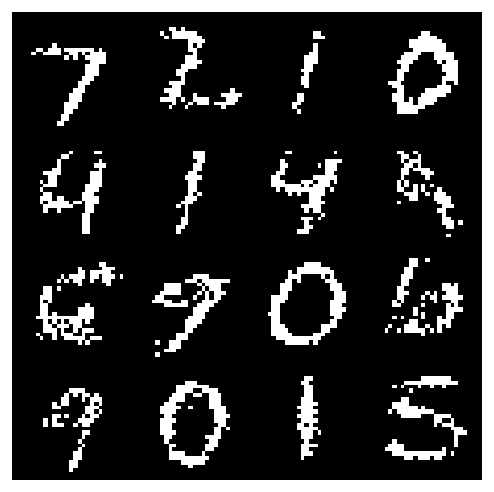
\includegraphics[width=\textwidth]{ex4_1_rbm_samples.pdf}
    \caption{RBM}
    \label{fig:ex4_1_rbm_samples}
  \end{subfigure}
  \begin{subfigure}{0.49\textwidth}
    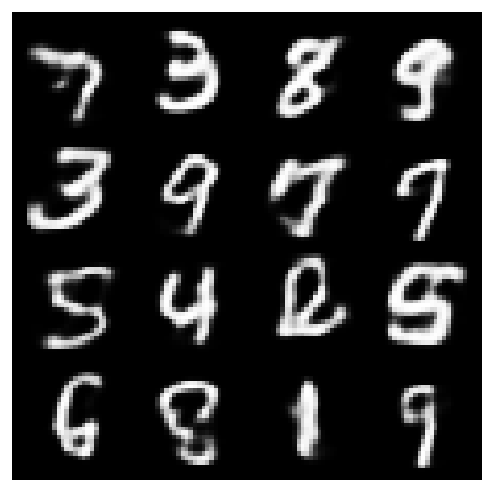
\includegraphics[width=\textwidth]{ex4_1_dbm_samples.pdf}
    \caption{DBM}
    \label{fig:ex4_1_dbm_samples}
  \end{subfigure}
  \caption{Samples generated after 1 Gibbs sampling step.}
  \label{fig:ex4_1_samples}
\end{figure}

The samples generated by the RBM and the DBM after 1 Gibbs sampling step are shown in
Figure~\ref{fig:ex4_1_samples}. The samples of the DBM are of higher quality than the samples of the
RBM, because they resemble digits more closely and have less artifacts. The biggest difference is
that the RBM only produces binary pixel values, while the digits of the DBM have continuous edges,
like anti-aliasing was applied. Also, the structure of the digits is more consistent in the DBM
samples.


\subsection{Generator and Discriminator in the Ring}
\label{ex:4.2}

\begin{task}{4.2.1}
  % Explain the different losses and results in the context of the GAN framework.
\end{task}

The loss of the generator measures how good the generator is at fooling the discriminator. The
generator tries to minimize this loss by generating samples that are similar to the real data. The
loss of the discriminator measures how good the discriminator is at distinguishing between real and
fake samples. The discriminator tries to minimize this loss by correctly classifying the samples.


\begin{task}{4.2.2}
  % What would you expect if the discriminator performs proportionally much better than the
  % generator?
\end{task}

If the discriminator performs much better than the generator, the generator will have a hard time
fooling the discriminator. This could lead to mode collapse, where the generator only produces a few
different samples. The generator will not be able to learn from the feedback of the discriminator.


\begin{task}{4.2.3}
  % Discuss and illustrate the convergence and stability of GANs.
\end{task}

The losses of the generator and discriminator during training are shown in
Figure~\ref{fig:ex4_2_gan_loss}. In the optimal case, both losses should converge to a low value, so
that the generator and discriminator reach an equilibrium. The losses should be balanced, so that
the generator can learn from the feedback of the discriminator. In this case, the losses of the
generator increase. However, this does not mean that the generator is getting worse, because the
discriminator is also getting better.\\
If the losses of the generator and discriminator are not balanced, the generator will not be able to
learn from the feedback of the discriminator. This could lead to mode collapse, where the generator
only produces a few different samples.


\begin{task}{4.2.4}
  % Explore the latent space and discuss.
\end{task}

A batch of random samples generated by the GAN is shown in Figure~\ref{fig:ex4_2_samples}. Most of
the samples resemble the digit $0$. The structure of the digits is clear for about half of the
samples. The model seems to prefer round shapes, as there are only a few samples that could be
interpreted as a $4$ or $7$ and none that could be interpreted as a $1$. Also, all samples have
a noisy background, some more than others.


\begin{task}{4.2.5}
  % Try the CNN-based backbone and discuss.
\end{task}

\begin{figure}[ht]
  \centering
  \begin{subfigure}{0.49\textwidth}
    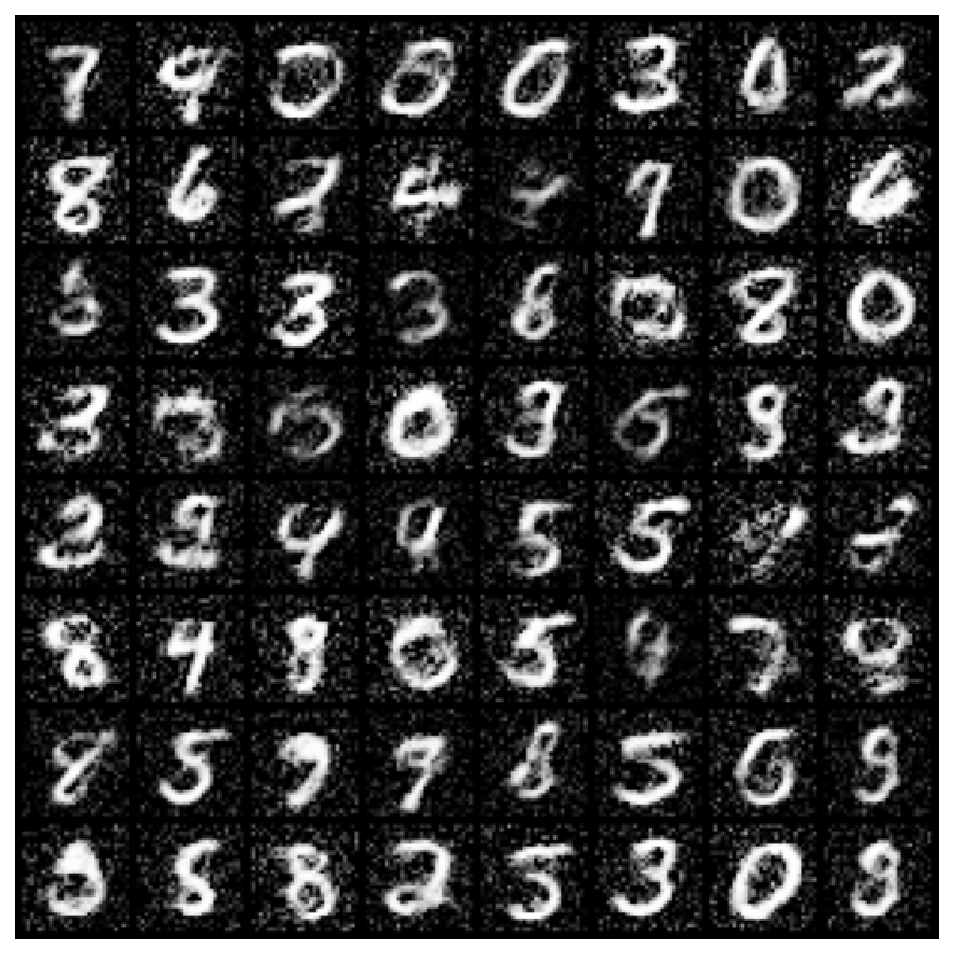
\includegraphics[width=\textwidth]{ex4_2_samples_vanilla.pdf}
    \caption{Feedforward backbone}
    \label{fig:ex4_2_samples_vanilla}
  \end{subfigure}
  \begin{subfigure}{0.49\textwidth}
    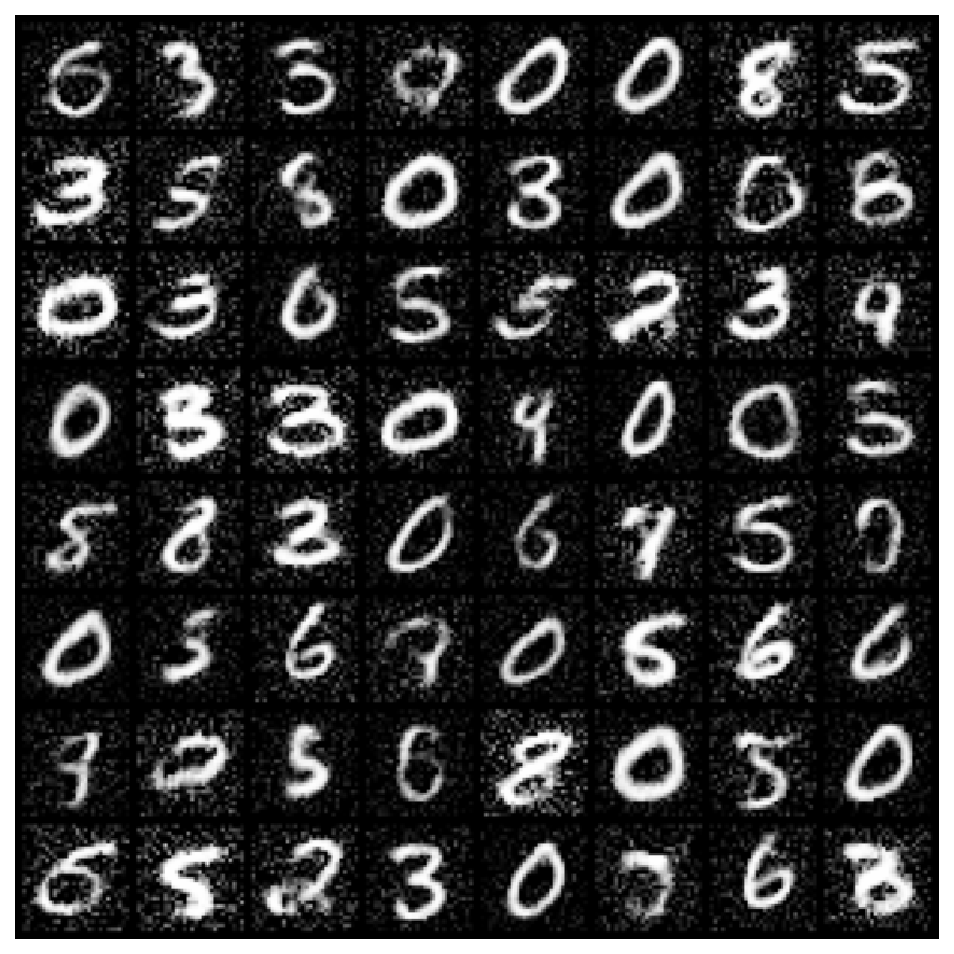
\includegraphics[width=\textwidth]{ex4_2_samples_cnn.pdf}
    \caption{CNN backbone}
    \label{fig:ex4_2_samples_cnn}
  \end{subfigure}
  \caption{Samples generated by the GAN with different backbones.}
  \label{fig:ex4_2_samples}
\end{figure}

A comparison of the samples generated by the GAN with the different backbones is shown in
Figure~\ref{fig:ex4_2_samples}. In general, the samples generated by the CNN backbone are of higher
quality. The structure of the digits is clearer and the background is less noisy. There are only a
few samples that are hardly recognizable as digits. The CNN backbone also prefers round shapes and
the digit $0$ is also the most common digit.


\begin{task}{4.2.6}
  % What are the advantages and disadvantages of GAN-models compared to other generative models,
  % e.g. the auto-encoder family or diffusion models? Think about the conceptual aspects, the
  % quality of the results, the training considerations, etc.
\end{task}

The main advantage of GANs is that they can generate samples that are very realistic, due to the
adversarial training. However, GANs are hard to train and can be unstable. They are also prone to
mode collapse, like described above. Auto-encoders are easier to train and can also be used for
dimensionality reduction. However, they are not as good at generating realistic samples. Diffusion
models are also good at generating realistic samples, but they need longer to train. They are also
harder to understand than GANs.



\subsection{An Auto-Encoder With a Touch}
\label{ex:4.3}

\begin{task}{4.3.1}
  % In practice, the model does not maximize the log-likelihood but another metric. Which one? Why
  % is that and how does it work?
\end{task}

The model maximizes the evidence lower bound (ELBO) instead of the log-likelihood. The ELBO is the
sum of the (negative) reconstruction error and the Kullback-Leibler divergence between the latent
distribution and the prior distribution. The reconstruction error expresses how good the model is at
reconstructing the input data. The KL-divergence measures how much information is lost when the
latent distribution is approximated by the prior distribution.\\
The ELBO is used because it is easier to optimize than the log-likelihood. Also, the KL-divergence
term acts as a regularizer that prevents the model from overfitting.


\begin{task}{4.3.2}
  % In particular, what similarities and differences do you see when compared with stacked
  % auto-encoder from the previous assignment? What is the metric for the reconstruction error in
  % each case?
\end{task}

The main difference between the stacked auto-encoder and the VAE is that the VAE uses a
probabilistic approach to model the latent space. This allows the VAE to generate new samples by
sampling from the latent space. The stacked auto-encoder uses cross entropy and the VAE uses binary
cross entropy as the metric for the reconstruction error.


\begin{task}{4.3.3}
  % Explore the latent space using the provided code and discuss what you observe.
\end{task}

\begin{figure}[t]
  \centering
  \begin{minipage}{0.6\textwidth}
    \centering
    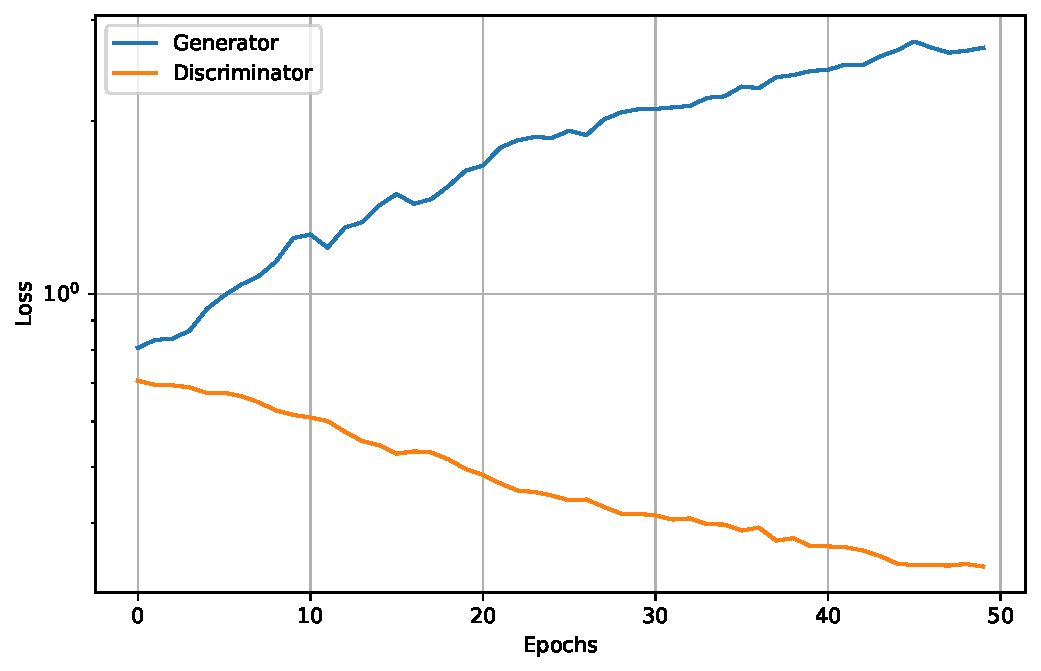
\includegraphics[width=0.9\linewidth]{ex4_2_gan_loss.pdf}
    \captionof{figure}{Losses of the generator and discriminator during training.}
    \label{fig:ex4_2_gan_loss}
  \end{minipage}
  \begin{minipage}{0.39\textwidth}
    \centering
    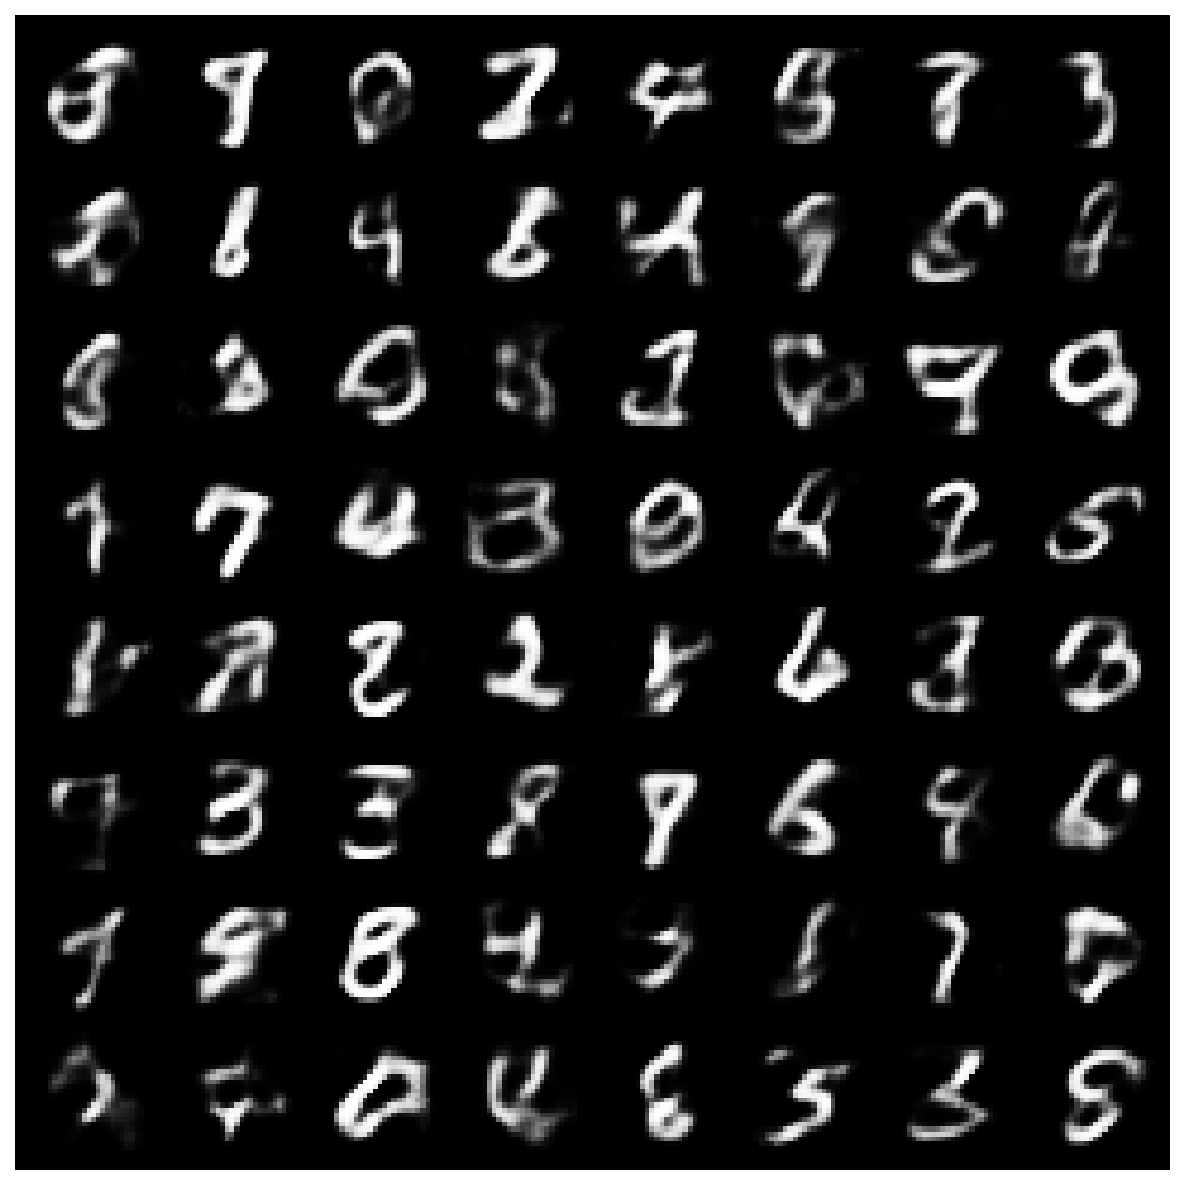
\includegraphics[width=0.9\linewidth]{ex4_3_samples.pdf}
    \captionof{figure}{Random samples from the latent space of the VAE.}
    \label{fig:ex4_3_samples}
  \end{minipage}
\end{figure}

I trained the VAE with latent-space dimension $300$ and middle layer dimension $1024$ for $100$
epochs. The samples from the latent space are shown in Figure~\ref{fig:ex4_3_samples}. One can tell
that they are supposed to be digits, but only a few of them have a clear structure. There are some
samples that are not recognizable as digits at all. Others can be seen as a digit, but are not
clearly defined. A big majority of the outputs look like the digit $8$. Also, there is no sample
that is clearly a $0$-digit. I consider this as counterintuitive, because of its simple shape.


\begin{task}{4.3.4}
  % Compare the generation mechanism to GANs. You may optionally want to consider similar backbones
  % for a fair comparison. What are the advantages and disadvantages?
\end{task}

The VAE generates samples by sampling from the latent space, while the GAN generates samples by
feeding random noise through the generator. The VAE has the advantage that it can generate samples
from the latent space, while the GAN can only generate samples from the input space. This makes the
VAE more interpretable, because you can see how the latent space is structured. The GAN has the
advantage that it can generate more realistic samples, because it is trained to fool the
discriminator.